\documentclass[]{book}
\usepackage{lmodern}
\usepackage{amssymb,amsmath}
\usepackage{ifxetex,ifluatex}
\usepackage{fixltx2e} % provides \textsubscript
\ifnum 0\ifxetex 1\fi\ifluatex 1\fi=0 % if pdftex
  \usepackage[T1]{fontenc}
  \usepackage[utf8]{inputenc}
\else % if luatex or xelatex
  \ifxetex
    \usepackage{mathspec}
  \else
    \usepackage{fontspec}
  \fi
  \defaultfontfeatures{Ligatures=TeX,Scale=MatchLowercase}
\fi
% use upquote if available, for straight quotes in verbatim environments
\IfFileExists{upquote.sty}{\usepackage{upquote}}{}
% use microtype if available
\IfFileExists{microtype.sty}{%
\usepackage{microtype}
\UseMicrotypeSet[protrusion]{basicmath} % disable protrusion for tt fonts
}{}
\usepackage[margin=1in]{geometry}
\usepackage{hyperref}
\hypersetup{unicode=true,
            pdftitle={Exploring data using R},
            pdfauthor={Kamarul Imran Musa, Wan Nor Arifin},
            pdfborder={0 0 0},
            breaklinks=true}
\urlstyle{same}  % don't use monospace font for urls
\usepackage{color}
\usepackage{fancyvrb}
\newcommand{\VerbBar}{|}
\newcommand{\VERB}{\Verb[commandchars=\\\{\}]}
\DefineVerbatimEnvironment{Highlighting}{Verbatim}{commandchars=\\\{\}}
% Add ',fontsize=\small' for more characters per line
\usepackage{framed}
\definecolor{shadecolor}{RGB}{248,248,248}
\newenvironment{Shaded}{\begin{snugshade}}{\end{snugshade}}
\newcommand{\KeywordTok}[1]{\textcolor[rgb]{0.13,0.29,0.53}{\textbf{{#1}}}}
\newcommand{\DataTypeTok}[1]{\textcolor[rgb]{0.13,0.29,0.53}{{#1}}}
\newcommand{\DecValTok}[1]{\textcolor[rgb]{0.00,0.00,0.81}{{#1}}}
\newcommand{\BaseNTok}[1]{\textcolor[rgb]{0.00,0.00,0.81}{{#1}}}
\newcommand{\FloatTok}[1]{\textcolor[rgb]{0.00,0.00,0.81}{{#1}}}
\newcommand{\ConstantTok}[1]{\textcolor[rgb]{0.00,0.00,0.00}{{#1}}}
\newcommand{\CharTok}[1]{\textcolor[rgb]{0.31,0.60,0.02}{{#1}}}
\newcommand{\SpecialCharTok}[1]{\textcolor[rgb]{0.00,0.00,0.00}{{#1}}}
\newcommand{\StringTok}[1]{\textcolor[rgb]{0.31,0.60,0.02}{{#1}}}
\newcommand{\VerbatimStringTok}[1]{\textcolor[rgb]{0.31,0.60,0.02}{{#1}}}
\newcommand{\SpecialStringTok}[1]{\textcolor[rgb]{0.31,0.60,0.02}{{#1}}}
\newcommand{\ImportTok}[1]{{#1}}
\newcommand{\CommentTok}[1]{\textcolor[rgb]{0.56,0.35,0.01}{\textit{{#1}}}}
\newcommand{\DocumentationTok}[1]{\textcolor[rgb]{0.56,0.35,0.01}{\textbf{\textit{{#1}}}}}
\newcommand{\AnnotationTok}[1]{\textcolor[rgb]{0.56,0.35,0.01}{\textbf{\textit{{#1}}}}}
\newcommand{\CommentVarTok}[1]{\textcolor[rgb]{0.56,0.35,0.01}{\textbf{\textit{{#1}}}}}
\newcommand{\OtherTok}[1]{\textcolor[rgb]{0.56,0.35,0.01}{{#1}}}
\newcommand{\FunctionTok}[1]{\textcolor[rgb]{0.00,0.00,0.00}{{#1}}}
\newcommand{\VariableTok}[1]{\textcolor[rgb]{0.00,0.00,0.00}{{#1}}}
\newcommand{\ControlFlowTok}[1]{\textcolor[rgb]{0.13,0.29,0.53}{\textbf{{#1}}}}
\newcommand{\OperatorTok}[1]{\textcolor[rgb]{0.81,0.36,0.00}{\textbf{{#1}}}}
\newcommand{\BuiltInTok}[1]{{#1}}
\newcommand{\ExtensionTok}[1]{{#1}}
\newcommand{\PreprocessorTok}[1]{\textcolor[rgb]{0.56,0.35,0.01}{\textit{{#1}}}}
\newcommand{\AttributeTok}[1]{\textcolor[rgb]{0.77,0.63,0.00}{{#1}}}
\newcommand{\RegionMarkerTok}[1]{{#1}}
\newcommand{\InformationTok}[1]{\textcolor[rgb]{0.56,0.35,0.01}{\textbf{\textit{{#1}}}}}
\newcommand{\WarningTok}[1]{\textcolor[rgb]{0.56,0.35,0.01}{\textbf{\textit{{#1}}}}}
\newcommand{\AlertTok}[1]{\textcolor[rgb]{0.94,0.16,0.16}{{#1}}}
\newcommand{\ErrorTok}[1]{\textcolor[rgb]{0.64,0.00,0.00}{\textbf{{#1}}}}
\newcommand{\NormalTok}[1]{{#1}}
\usepackage{longtable,booktabs}
\usepackage{graphicx,grffile}
\makeatletter
\def\maxwidth{\ifdim\Gin@nat@width>\linewidth\linewidth\else\Gin@nat@width\fi}
\def\maxheight{\ifdim\Gin@nat@height>\textheight\textheight\else\Gin@nat@height\fi}
\makeatother
% Scale images if necessary, so that they will not overflow the page
% margins by default, and it is still possible to overwrite the defaults
% using explicit options in \includegraphics[width, height, ...]{}
\setkeys{Gin}{width=\maxwidth,height=\maxheight,keepaspectratio}
\IfFileExists{parskip.sty}{%
\usepackage{parskip}
}{% else
\setlength{\parindent}{0pt}
\setlength{\parskip}{6pt plus 2pt minus 1pt}
}
\setlength{\emergencystretch}{3em}  % prevent overfull lines
\providecommand{\tightlist}{%
  \setlength{\itemsep}{0pt}\setlength{\parskip}{0pt}}
\setcounter{secnumdepth}{5}
% Redefines (sub)paragraphs to behave more like sections
\ifx\paragraph\undefined\else
\let\oldparagraph\paragraph
\renewcommand{\paragraph}[1]{\oldparagraph{#1}\mbox{}}
\fi
\ifx\subparagraph\undefined\else
\let\oldsubparagraph\subparagraph
\renewcommand{\subparagraph}[1]{\oldsubparagraph{#1}\mbox{}}
\fi

%%% Use protect on footnotes to avoid problems with footnotes in titles
\let\rmarkdownfootnote\footnote%
\def\footnote{\protect\rmarkdownfootnote}

%%% Change title format to be more compact
\usepackage{titling}

% Create subtitle command for use in maketitle
\newcommand{\subtitle}[1]{
  \posttitle{
    \begin{center}\large#1\end{center}
    }
}

\setlength{\droptitle}{-2em}
  \title{Exploring data using R}
  \pretitle{\vspace{\droptitle}\centering\huge}
  \posttitle{\par}
  \author{Kamarul Imran Musa, Wan Nor Arifin}
  \preauthor{\centering\large\emph}
  \postauthor{\par}
  \predate{\centering\large\emph}
  \postdate{\par}
  \date{2017-07-13}


\usepackage{amsthm}
\newtheorem{theorem}{Theorem}[chapter]
\newtheorem{lemma}{Lemma}[chapter]
\theoremstyle{definition}
\newtheorem{definition}{Definition}[chapter]
\newtheorem{corollary}{Corollary}[chapter]
\newtheorem{proposition}{Proposition}[chapter]
\theoremstyle{definition}
\newtheorem{example}{Example}[chapter]
\theoremstyle{remark}
\newtheorem*{remark}{Remark}
\begin{document}
\maketitle

{
\setcounter{tocdepth}{1}
\tableofcontents
}
\chapter{Introduction to R}\label{introduction-to-r}

This chapter introduces readers to the basics of working with data in R.
We will start with installing R in your computer and getting familiar
with RStudio interface. These will be followed by the basics of handling
data in R.

\section{R and RStudio}\label{r-and-rstudio}

\subsection{Installation of R}\label{installation-of-r}

\begin{itemize}
\tightlist
\item
  The latest version of R is R version 3.4.1 (2017-06-30), Single
  Candle.
\item
  R is available for Windows, Mac OS and Linux.
\item
  The installation files can be downloaded from
  \url{https://cran.r-project.org/}.
\item
  Users can install different versions of R in a same machine or
  computer.
\item
  There is no need to uninstall if you want to upgrade the currently
  installed R.
\end{itemize}

\subsection{Starting R}\label{starting-r}

Double click on R icon and you should get this

You should see an R console.

\subsection{Installation of RStudio}\label{installation-of-rstudio}

RStudio installation files can be downloaded from
\url{http://www.rstudio.com/}. First, make sure you have RStudio
successfully installed.

\subsubsection{Starting RStudio}\label{starting-rstudio}

You can double click on RStudio icon and you will see this:

\subsubsection{Why RStudio?}\label{why-rstudio}

\begin{itemize}
\tightlist
\item
  Working with R console is alright.
\item
  But for many people, they prefer to communicate with R using a
  graphical user interface (GUI).
\item
  RStudio is the popular GUI and intergrated developement environment
  (IDE) for R.
\item
  Other R IDE includes Microsoft R
\end{itemize}

Check this links for more info:

\begin{enumerate}
\def\labelenumi{\arabic{enumi}.}
\tightlist
\item
  RStudio \url{https://www.rstudio.com/}
\item
  Microsoft R
  \url{http://blog.revolutionanalytics.com/2016/01/microsoft-r-open.html}
\end{enumerate}

\subsubsection{RStudio interface}\label{rstudio-interface}

You should be able to see 4 panes in the layout. You should see that

\begin{enumerate}
\def\labelenumi{\arabic{enumi}.}
\tightlist
\item
  Console - the lower left pane. It tells you about your R information.
\item
  Source - the upper left pane. It shows the active files.
\item
  Environment and History - the upper right pane. It shows the currently
  loaded data files and values, and command history.
\item
  Miscellaneous - the lower right pane. It contains most important tabs,
  which are Files, Plots, Packages, Help and Viewer. It list file names,
  show plots, show packages, display help document and view outputs.
\end{enumerate}

\section{Working with packages}\label{working-with-packages}

\subsection{About packages}\label{about-packages}

R uses packages to perform its tasks.

There are two common packages:

\begin{enumerate}
\def\labelenumi{\arabic{enumi}.}
\tightlist
\item
  \texttt{base} packages
\item
  \texttt{user-contributed} packages
\end{enumerate}

\begin{itemize}
\tightlist
\item
  The base packages come with the installation of R
\item
  The base package provides basic but adequate functions to perform many
  standard data management, visualization and analysis.
\item
  However, user needs to install user-contributed packages if they need
  to perform functions (tasks) not available in the base package
\item
  User-contributed packages allow users to perform more advanced and
  more complicated functions
\item
  There are more than 10200 packages as of March 2017
\end{itemize}

For a complete list of packages, see
\url{https://cran.r-project.org/web/packages/}

\subsection{Package installation}\label{package-installation}

You can install user-contributed packages through:

\begin{enumerate}
\def\labelenumi{\arabic{enumi}.}
\tightlist
\item
  Internet (to cran)
\item
  Github packages
\item
  Local zip files
\end{enumerate}

We will learn to install a few small packages.

Basically, a function to install a package will look like this

\begin{Shaded}
\begin{Highlighting}[]
\KeywordTok{install.packages}\NormalTok{(}\StringTok{"package.name"}\NormalTok{)}
\end{Highlighting}
\end{Shaded}

To install a package, saya \texttt{car} 1. put your cursor in the
CONSOLE pane 2. type the codes below

\begin{Shaded}
\begin{Highlighting}[]
\KeywordTok{install.packages}\NormalTok{(}\StringTok{"car"}\NormalTok{)}
\end{Highlighting}
\end{Shaded}

\begin{enumerate}
\def\labelenumi{\arabic{enumi}.}
\setcounter{enumi}{2}
\tightlist
\item
  press Ctrl + ENTER
\end{enumerate}

\subsection{Loading packages}\label{loading-packages}

Basically, to utilize a package, it has to be loaded using
\texttt{library()} function,

\begin{Shaded}
\begin{Highlighting}[]
\KeywordTok{library}\NormalTok{(}\StringTok{"package.name"}\NormalTok{)}
\end{Highlighting}
\end{Shaded}

For example, we load the newly installed \texttt{car} package

\begin{Shaded}
\begin{Highlighting}[]
\KeywordTok{library}\NormalTok{(}\StringTok{"haven"}\NormalTok{)}
\end{Highlighting}
\end{Shaded}

\section{Working directory}\label{working-directory}

In general, R reads and saves data and other files into a working
directory. Therefore, a user must create or specify the working
directory to work with R. This is a good practice.

A working directory:

\begin{enumerate}
\def\labelenumi{\arabic{enumi}.}
\tightlist
\item
  stores all the outputs such as the plots, html files, pdf files
\item
  contains your data
\end{enumerate}

Creating a working directory is a simple BUT an important step.

Unfortunately, many users do not pay attention to this and forget to set
it. So, remember, this is a very important step to work in R.

\subsection{Setting a working
directory}\label{setting-a-working-directory}

To set your working directory:

\begin{enumerate}
\def\labelenumi{\arabic{enumi}.}
\tightlist
\item
  Go back to RStudio's Miscellaneous pane.
\item
  In the Files tab, click \emph{\ldots{}}
\item
  Navigate to the folder containing your data or any folder you want to
  work in.
\item
  Click \emph{More}
\item
  Click \emph{Set as working directory}
\end{enumerate}

or simply use \texttt{setwd} function to do so.

\begin{Shaded}
\begin{Highlighting}[]
\KeywordTok{setwd}\NormalTok{(}\StringTok{"path to your folder"}\NormalTok{)}
\end{Highlighting}
\end{Shaded}

for example in Windows

\begin{Shaded}
\begin{Highlighting}[]
\KeywordTok{setwd}\NormalTok{(}\StringTok{"C:/myfolder"}\NormalTok{)}
\end{Highlighting}
\end{Shaded}

or in Mac OS/Linux

\begin{Shaded}
\begin{Highlighting}[]
\KeywordTok{setwd}\NormalTok{(}\StringTok{"~/myfolder"}\NormalTok{)}
\end{Highlighting}
\end{Shaded}

\section{Data management}\label{data-management}

This section is concerned with reading data from dataset and displaying
data.

\subsection{Reading data set}\label{reading-data-set}

Easiest is to read .csv file,

\begin{Shaded}
\begin{Highlighting}[]
\KeywordTok{read.csv}\NormalTok{(}\StringTok{"file.name"}\NormalTok{)}
\end{Highlighting}
\end{Shaded}

For SPSS file, need \texttt{foreign} package,

\begin{Shaded}
\begin{Highlighting}[]
\KeywordTok{library}\NormalTok{(}\StringTok{"foreign"}\NormalTok{)}
\KeywordTok{read.spss}\NormalTok{(}\StringTok{"file.name"}\NormalTok{)}
\end{Highlighting}
\end{Shaded}

Can read data in table format from text file. From text file,

\begin{Shaded}
\begin{Highlighting}[]
\KeywordTok{read.table}\NormalTok{(}\StringTok{"file.name"}\NormalTok{, }\DataTypeTok{header =} \OtherTok{TRUE}\NormalTok{)}
\end{Highlighting}
\end{Shaded}

\subsection{Viewing data set}\label{viewing-data-set}

Easy, just type the name,

\begin{Shaded}
\begin{Highlighting}[]
\NormalTok{data}
\end{Highlighting}
\end{Shaded}

Nicer, using \texttt{View()}

\begin{Shaded}
\begin{Highlighting}[]
\KeywordTok{View}\NormalTok{(data)}
\end{Highlighting}
\end{Shaded}

Important tasks

\begin{Shaded}
\begin{Highlighting}[]
\KeywordTok{dim}\NormalTok{(data)}
\KeywordTok{str}\NormalTok{(data)}
\KeywordTok{names}\NormalTok{(data)}
\end{Highlighting}
\end{Shaded}

\section{More about data management}\label{more-about-data-management}

In this section, we will deal with more advanced data management
(subsetting, recoding and creating new variables) and direct data entry
(especially useful for tables).

\subsection{Subsetting}\label{subsetting}

\subsection{Recoding}\label{recoding}

\subsection{Creating new variables}\label{creating-new-variables}

\subsection{Direct data entry}\label{direct-data-entry}

\chapter{Textual}\label{textual}

In this chapter, we will go through a number of R functions for basic
statistics. The focus will be on the results that are presented in form
of numbers in text or tables (textual). We will mostly use the builtin
functions (from R standard library). Extra packages will be introduced
whenever necessary.

\section{Basic descriptive
statistics}\label{basic-descriptive-statistics}

In this part, we are going to use the functions as applied to a
variable. For this purpose, we are going to use builtin datasets in R.
You can view the available datasets by

\begin{Shaded}
\begin{Highlighting}[]
\KeywordTok{data}\NormalTok{()}
\end{Highlighting}
\end{Shaded}

\begin{Shaded}
\begin{Highlighting}[]
\NormalTok{## Data sets in package ‘datasets’:}

\NormalTok{## AirPassengers                     Monthly Airline Passenger Numbers 1949-1960}
\NormalTok{## BJsales                           Sales Data with Leading Indicator}
\NormalTok{## BJsales.lead (BJsales)            Sales Data with Leading Indicator}
\NormalTok{## BOD                               Biochemical Oxygen Demand}
\NormalTok{## CO2                               Carbon Dioxide Uptake in Grass Plants}
\NormalTok{## ...}
\end{Highlighting}
\end{Shaded}

We can view any dataset description by appending ``?'' to the dataset
name. For example,

\begin{Shaded}
\begin{Highlighting}[]
\NormalTok{?chickwts}
\end{Highlighting}
\end{Shaded}

We will start by using \texttt{chickwts} dataset that contains both
numerical (\texttt{weight}) and categorical (\texttt{feed}) variables.
We can view the first six observations,

\begin{Shaded}
\begin{Highlighting}[]
\KeywordTok{head}\NormalTok{(chickwts)}
\end{Highlighting}
\end{Shaded}

\begin{verbatim}
##   weight      feed
## 1    179 horsebean
## 2    160 horsebean
## 3    136 horsebean
## 4    227 horsebean
## 5    217 horsebean
## 6    168 horsebean
\end{verbatim}

the last six observations,

\begin{Shaded}
\begin{Highlighting}[]
\KeywordTok{tail}\NormalTok{(chickwts)}
\end{Highlighting}
\end{Shaded}

\begin{verbatim}
##    weight   feed
## 66    352 casein
## 67    359 casein
## 68    216 casein
## 69    222 casein
## 70    283 casein
## 71    332 casein
\end{verbatim}

and the dimension of the data (row and column).

\begin{Shaded}
\begin{Highlighting}[]
\KeywordTok{dim}\NormalTok{(chickwts)}
\end{Highlighting}
\end{Shaded}

\begin{verbatim}
## [1] 71  2
\end{verbatim}

Here we have 71 rows (71 subjects) and two columns (two variables).

Next, view the names of the variables,

\begin{Shaded}
\begin{Highlighting}[]
\KeywordTok{names}\NormalTok{(chickwts)}
\end{Highlighting}
\end{Shaded}

\begin{verbatim}
## [1] "weight" "feed"
\end{verbatim}

and view the details of the data,

\begin{Shaded}
\begin{Highlighting}[]
\KeywordTok{str}\NormalTok{(chickwts)}
\end{Highlighting}
\end{Shaded}

\begin{verbatim}
## 'data.frame':    71 obs. of  2 variables:
##  $ weight: num  179 160 136 227 217 168 108 124 143 140 ...
##  $ feed  : Factor w/ 6 levels "casein","horsebean",..: 2 2 2 2 2 2 2 2 2 2 ...
\end{verbatim}

which shows that \texttt{weight} is a numerical variable and
\texttt{feed} is a factor, i.e.~a categorical variable. \texttt{feed}
consists of six categories or levels.

We can view the levels in \texttt{feed},

\begin{Shaded}
\begin{Highlighting}[]
\KeywordTok{levels}\NormalTok{(chickwts$feed)}
\end{Highlighting}
\end{Shaded}

\begin{verbatim}
## [1] "casein"    "horsebean" "linseed"   "meatmeal"  "soybean"   "sunflower"
\end{verbatim}

\subsection{Describing a numerical
variable}\label{describing-a-numerical-variable}

A numberical variable is described by a number of descriptive statistics
below.

To judge the central tendency of the \texttt{weight} variable, we obtain
its mean,

\begin{Shaded}
\begin{Highlighting}[]
\KeywordTok{mean}\NormalTok{(chickwts$weight)}
\end{Highlighting}
\end{Shaded}

\begin{verbatim}
## [1] 261.3099
\end{verbatim}

and median,

\begin{Shaded}
\begin{Highlighting}[]
\KeywordTok{median}\NormalTok{(chickwts$weight)}
\end{Highlighting}
\end{Shaded}

\begin{verbatim}
## [1] 258
\end{verbatim}

To judge its spread and variability, we can view its minimum, maximum
and range

\begin{Shaded}
\begin{Highlighting}[]
\KeywordTok{min}\NormalTok{(chickwts$weight)}
\end{Highlighting}
\end{Shaded}

\begin{verbatim}
## [1] 108
\end{verbatim}

\begin{Shaded}
\begin{Highlighting}[]
\KeywordTok{max}\NormalTok{(chickwts$weight)}
\end{Highlighting}
\end{Shaded}

\begin{verbatim}
## [1] 423
\end{verbatim}

\begin{Shaded}
\begin{Highlighting}[]
\KeywordTok{range}\NormalTok{(chickwts$weight)}
\end{Highlighting}
\end{Shaded}

\begin{verbatim}
## [1] 108 423
\end{verbatim}

and obtain its standard deviation (SD)

\begin{Shaded}
\begin{Highlighting}[]
\KeywordTok{sd}\NormalTok{(chickwts$weight)}
\end{Highlighting}
\end{Shaded}

\begin{verbatim}
## [1] 78.0737
\end{verbatim}

variance,

\begin{Shaded}
\begin{Highlighting}[]
\KeywordTok{var}\NormalTok{(chickwts$weight)}
\end{Highlighting}
\end{Shaded}

\begin{verbatim}
## [1] 6095.503
\end{verbatim}

quantile,

\begin{Shaded}
\begin{Highlighting}[]
\KeywordTok{quantile}\NormalTok{(chickwts$weight)}
\end{Highlighting}
\end{Shaded}

\begin{verbatim}
##    0%   25%   50%   75%  100% 
## 108.0 204.5 258.0 323.5 423.0
\end{verbatim}

and interquartile range (IQR)

\begin{Shaded}
\begin{Highlighting}[]
\KeywordTok{IQR}\NormalTok{(chickwts$weight)}
\end{Highlighting}
\end{Shaded}

\begin{verbatim}
## [1] 119
\end{verbatim}

There are nine types of quantile algorithms in R (for \texttt{quantile}
and \texttt{IQR}), the default being type 7. You may change this to type
6 (Minitab and SPSS),

\begin{Shaded}
\begin{Highlighting}[]
\KeywordTok{quantile}\NormalTok{(chickwts$weight, }\DataTypeTok{type =} \DecValTok{6}\NormalTok{)}
\end{Highlighting}
\end{Shaded}

\begin{verbatim}
##   0%  25%  50%  75% 100% 
##  108  203  258  325  423
\end{verbatim}

\begin{Shaded}
\begin{Highlighting}[]
\KeywordTok{IQR}\NormalTok{(chickwts$weight, }\DataTypeTok{type =} \DecValTok{6}\NormalTok{)}
\end{Highlighting}
\end{Shaded}

\begin{verbatim}
## [1] 122
\end{verbatim}

In addition to SD and IQR, we can obtain its median absolute deviation
(MAD),

\begin{Shaded}
\begin{Highlighting}[]
\KeywordTok{mad}\NormalTok{(chickwts$weight)}
\end{Highlighting}
\end{Shaded}

\begin{verbatim}
## [1] 91.9212
\end{verbatim}

It is actually simpler to obtain most these in a single command,

\begin{Shaded}
\begin{Highlighting}[]
\KeywordTok{summary}\NormalTok{(chickwts$weight)}
\end{Highlighting}
\end{Shaded}

\begin{verbatim}
##    Min. 1st Qu.  Median    Mean 3rd Qu.    Max. 
##   108.0   204.5   258.0   261.3   323.5   423.0
\end{verbatim}

even simpler, obtain all of the statistics using \texttt{describe} in
the \texttt{psych} package

\begin{Shaded}
\begin{Highlighting}[]
\KeywordTok{install.packages}\NormalTok{(}\StringTok{"psych"}\NormalTok{)}
\end{Highlighting}
\end{Shaded}

\begin{Shaded}
\begin{Highlighting}[]
\KeywordTok{library}\NormalTok{(psych)}
\KeywordTok{describe}\NormalTok{(chickwts$weight)}
\end{Highlighting}
\end{Shaded}

\begin{verbatim}
##    vars  n   mean    sd median trimmed   mad min max range  skew kurtosis
## X1    1 71 261.31 78.07    258     261 91.92 108 423   315 -0.01    -0.97
##      se
## X1 9.27
\end{verbatim}

\subsection{Describing a categorical
variable}\label{describing-a-categorical-variable}

A categorical variable is described by its count, proportion and
percentage by categories.

We obtain the count of the \texttt{feed} variable,

\begin{Shaded}
\begin{Highlighting}[]
\KeywordTok{summary}\NormalTok{(chickwts$feed)}
\end{Highlighting}
\end{Shaded}

\begin{verbatim}
##    casein horsebean   linseed  meatmeal   soybean sunflower 
##        12        10        12        11        14        12
\end{verbatim}

\begin{Shaded}
\begin{Highlighting}[]
\KeywordTok{table}\NormalTok{(chickwts$feed)}
\end{Highlighting}
\end{Shaded}

\begin{verbatim}
## 
##    casein horsebean   linseed  meatmeal   soybean sunflower 
##        12        10        12        11        14        12
\end{verbatim}

both \texttt{summary} and \texttt{table} give the same result.

\texttt{prop.table} gives the proportion of the result from the count.

\begin{Shaded}
\begin{Highlighting}[]
\KeywordTok{prop.table}\NormalTok{(}\KeywordTok{table}\NormalTok{(chickwts$feed))}
\end{Highlighting}
\end{Shaded}

\begin{verbatim}
## 
##    casein horsebean   linseed  meatmeal   soybean sunflower 
## 0.1690141 0.1408451 0.1690141 0.1549296 0.1971831 0.1690141
\end{verbatim}

the result can be easily turned into percentage,

\begin{Shaded}
\begin{Highlighting}[]
\KeywordTok{prop.table}\NormalTok{(}\KeywordTok{table}\NormalTok{(chickwts$feed))*}\DecValTok{100}
\end{Highlighting}
\end{Shaded}

\begin{verbatim}
## 
##    casein horsebean   linseed  meatmeal   soybean sunflower 
##  16.90141  14.08451  16.90141  15.49296  19.71831  16.90141
\end{verbatim}

To view the count and the percentage together, we can use
\texttt{cbind},

\begin{Shaded}
\begin{Highlighting}[]
\KeywordTok{cbind}\NormalTok{(}\DataTypeTok{n =} \KeywordTok{table}\NormalTok{(chickwts$feed), }\StringTok{"%"} \NormalTok{=}\StringTok{ }\KeywordTok{prop.table}\NormalTok{(}\KeywordTok{table}\NormalTok{(chickwts$feed))*}\DecValTok{100}\NormalTok{)}
\end{Highlighting}
\end{Shaded}

\begin{verbatim}
##            n        %
## casein    12 16.90141
## horsebean 10 14.08451
## linseed   12 16.90141
## meatmeal  11 15.49296
## soybean   14 19.71831
## sunflower 12 16.90141
\end{verbatim}

We need the quotation marks " " around the percentage sign \%, because
\% also serves as a mathematical operator in R.

\section{More on descriptive
statistics}\label{more-on-descriptive-statistics}

Just now, we viewed all the statistics as applied to a variable. In this
part, we are going to view the statistics on a number of variables. This
includes viewing a group of numerical variables or categorical
variables, or a mixture of numerical and categorical variables. This is
relevant in a sense that, most of the time, we want to view everything
in one go (e.g.~the statistics of all items in a questionnaire), compare
the means of several groups and obtain cross-tabulation of categorical
variables.

\subsection{Describing numerical
variables}\label{describing-numerical-variables}

Let us use \texttt{women} dataset,

\begin{Shaded}
\begin{Highlighting}[]
\KeywordTok{head}\NormalTok{(women)}
\end{Highlighting}
\end{Shaded}

\begin{verbatim}
##   height weight
## 1     58    115
## 2     59    117
## 3     60    120
## 4     61    123
## 5     62    126
## 6     63    129
\end{verbatim}

\begin{Shaded}
\begin{Highlighting}[]
\KeywordTok{names}\NormalTok{(women)}
\end{Highlighting}
\end{Shaded}

\begin{verbatim}
## [1] "height" "weight"
\end{verbatim}

\begin{Shaded}
\begin{Highlighting}[]
\KeywordTok{str}\NormalTok{(women)}
\end{Highlighting}
\end{Shaded}

\begin{verbatim}
## 'data.frame':    15 obs. of  2 variables:
##  $ height: num  58 59 60 61 62 63 64 65 66 67 ...
##  $ weight: num  115 117 120 123 126 129 132 135 139 142 ...
\end{verbatim}

which consists of \texttt{weight} and \texttt{height} numerical
variables.

The variables can be easily viewed together by \texttt{summary},

\begin{Shaded}
\begin{Highlighting}[]
\KeywordTok{summary}\NormalTok{(women)}
\end{Highlighting}
\end{Shaded}

\begin{verbatim}
##      height         weight     
##  Min.   :58.0   Min.   :115.0  
##  1st Qu.:61.5   1st Qu.:124.5  
##  Median :65.0   Median :135.0  
##  Mean   :65.0   Mean   :136.7  
##  3rd Qu.:68.5   3rd Qu.:148.0  
##  Max.   :72.0   Max.   :164.0
\end{verbatim}

even better using \texttt{describe} (\texttt{psych}),

\begin{Shaded}
\begin{Highlighting}[]
\KeywordTok{describe}\NormalTok{(women)}
\end{Highlighting}
\end{Shaded}

\begin{verbatim}
##        vars  n   mean    sd median trimmed   mad min max range skew
## height    1 15  65.00  4.47     65   65.00  5.93  58  72    14 0.00
## weight    2 15 136.73 15.50    135  136.31 17.79 115 164    49 0.23
##        kurtosis   se
## height    -1.44 1.15
## weight    -1.34 4.00
\end{verbatim}

\subsection{Describing categorical
variables}\label{describing-categorical-variables}

Let us use \texttt{infert} dataset,

\begin{Shaded}
\begin{Highlighting}[]
\KeywordTok{head}\NormalTok{(infert)}
\end{Highlighting}
\end{Shaded}

\begin{verbatim}
##   education age parity induced case spontaneous stratum pooled.stratum
## 1    0-5yrs  26      6       1    1           2       1              3
## 2    0-5yrs  42      1       1    1           0       2              1
## 3    0-5yrs  39      6       2    1           0       3              4
## 4    0-5yrs  34      4       2    1           0       4              2
## 5   6-11yrs  35      3       1    1           1       5             32
## 6   6-11yrs  36      4       2    1           1       6             36
\end{verbatim}

\begin{Shaded}
\begin{Highlighting}[]
\KeywordTok{names}\NormalTok{(infert)}
\end{Highlighting}
\end{Shaded}

\begin{verbatim}
## [1] "education"      "age"            "parity"         "induced"       
## [5] "case"           "spontaneous"    "stratum"        "pooled.stratum"
\end{verbatim}

\begin{Shaded}
\begin{Highlighting}[]
\KeywordTok{str}\NormalTok{(infert)}
\end{Highlighting}
\end{Shaded}

\begin{verbatim}
## 'data.frame':    248 obs. of  8 variables:
##  $ education     : Factor w/ 3 levels "0-5yrs","6-11yrs",..: 1 1 1 1 2 2 2 2 2 2 ...
##  $ age           : num  26 42 39 34 35 36 23 32 21 28 ...
##  $ parity        : num  6 1 6 4 3 4 1 2 1 2 ...
##  $ induced       : num  1 1 2 2 1 2 0 0 0 0 ...
##  $ case          : num  1 1 1 1 1 1 1 1 1 1 ...
##  $ spontaneous   : num  2 0 0 0 1 1 0 0 1 0 ...
##  $ stratum       : int  1 2 3 4 5 6 7 8 9 10 ...
##  $ pooled.stratum: num  3 1 4 2 32 36 6 22 5 19 ...
\end{verbatim}

We notice that \texttt{induced}, \texttt{case} and \texttt{spontaneous}
are not yet set as categorical variables, thus we need to
\texttt{factor} the variables. We view the value labels in the dataset
description,

\begin{Shaded}
\begin{Highlighting}[]
\NormalTok{?infert}
\end{Highlighting}
\end{Shaded}

We label the values in the variables according to the description as

\begin{Shaded}
\begin{Highlighting}[]
\NormalTok{infert$induced =}\StringTok{ }\KeywordTok{factor}\NormalTok{(infert$induced, }\DataTypeTok{levels =} \DecValTok{0}\NormalTok{:}\DecValTok{2}\NormalTok{, }\DataTypeTok{labels =} \KeywordTok{c}\NormalTok{(}\StringTok{"0"}\NormalTok{, }\StringTok{"1"}\NormalTok{, }\StringTok{"2 or more"}\NormalTok{))}
\NormalTok{infert$case =}\StringTok{ }\KeywordTok{factor}\NormalTok{(infert$case, }\DataTypeTok{levels =} \DecValTok{0}\NormalTok{:}\DecValTok{1}\NormalTok{, }\DataTypeTok{labels =} \KeywordTok{c}\NormalTok{(}\StringTok{"control"}\NormalTok{, }\StringTok{"case"}\NormalTok{))}
\NormalTok{infert$spontaneous =}\StringTok{ }\KeywordTok{factor}\NormalTok{(infert$spontaneous, }\DataTypeTok{levels =} \DecValTok{0}\NormalTok{:}\DecValTok{2}\NormalTok{, }\DataTypeTok{labels =} \KeywordTok{c}\NormalTok{(}\StringTok{"0"}\NormalTok{, }\StringTok{"1"}\NormalTok{, }\StringTok{"2 or more"}\NormalTok{))}
\KeywordTok{str}\NormalTok{(infert)}
\end{Highlighting}
\end{Shaded}

\begin{verbatim}
## 'data.frame':    248 obs. of  8 variables:
##  $ education     : Factor w/ 3 levels "0-5yrs","6-11yrs",..: 1 1 1 1 2 2 2 2 2 2 ...
##  $ age           : num  26 42 39 34 35 36 23 32 21 28 ...
##  $ parity        : num  6 1 6 4 3 4 1 2 1 2 ...
##  $ induced       : Factor w/ 3 levels "0","1","2 or more": 2 2 3 3 2 3 1 1 1 1 ...
##  $ case          : Factor w/ 2 levels "control","case": 2 2 2 2 2 2 2 2 2 2 ...
##  $ spontaneous   : Factor w/ 3 levels "0","1","2 or more": 3 1 1 1 2 2 1 1 2 1 ...
##  $ stratum       : int  1 2 3 4 5 6 7 8 9 10 ...
##  $ pooled.stratum: num  3 1 4 2 32 36 6 22 5 19 ...
\end{verbatim}

and we now all these variables are turned into factors.

Again, the variables can be easily viewed together by \texttt{summary},

\begin{Shaded}
\begin{Highlighting}[]
\KeywordTok{summary}\NormalTok{(infert[}\KeywordTok{c}\NormalTok{(}\StringTok{"education"}\NormalTok{, }\StringTok{"induced"}\NormalTok{, }\StringTok{"case"}\NormalTok{, }\StringTok{"spontaneous"}\NormalTok{)])}
\end{Highlighting}
\end{Shaded}

\begin{verbatim}
##    education        induced         case        spontaneous 
##  0-5yrs : 12   0        :143   control:165   0        :141  
##  6-11yrs:120   1        : 68   case   : 83   1        : 71  
##  12+ yrs:116   2 or more: 37                 2 or more: 36
\end{verbatim}

We do not use \texttt{table} here in form of
\texttt{table(infert{[}c("education",\ "induced",\ "case",\ "spontaneous"){]})}
because \texttt{table} used in this form will give us 3-way
cross-tabulation instead of count per categories. Cross-tabulation of
categorical variables will be covered later.

To obtain the proportion and percentage results, we have to use
\texttt{lapply},

\begin{Shaded}
\begin{Highlighting}[]
\KeywordTok{lapply}\NormalTok{(infert[}\KeywordTok{c}\NormalTok{(}\StringTok{"education"}\NormalTok{, }\StringTok{"induced"}\NormalTok{, }\StringTok{"case"}\NormalTok{, }\StringTok{"spontaneous"}\NormalTok{)], }
       \NormalTok{function(x) }\KeywordTok{summary}\NormalTok{(x)/}\KeywordTok{length}\NormalTok{(x))}
\end{Highlighting}
\end{Shaded}

\begin{verbatim}
## $education
##    0-5yrs   6-11yrs   12+ yrs 
## 0.0483871 0.4838710 0.4677419 
## 
## $induced
##         0         1 2 or more 
## 0.5766129 0.2741935 0.1491935 
## 
## $case
##   control      case 
## 0.6653226 0.3346774 
## 
## $spontaneous
##         0         1 2 or more 
## 0.5685484 0.2862903 0.1451613
\end{verbatim}

\begin{Shaded}
\begin{Highlighting}[]
\KeywordTok{lapply}\NormalTok{(infert[}\KeywordTok{c}\NormalTok{(}\StringTok{"education"}\NormalTok{, }\StringTok{"induced"}\NormalTok{, }\StringTok{"case"}\NormalTok{, }\StringTok{"spontaneous"}\NormalTok{)], }
       \NormalTok{function(x) }\KeywordTok{summary}\NormalTok{(x)/}\KeywordTok{length}\NormalTok{(x)*}\DecValTok{100}\NormalTok{)}
\end{Highlighting}
\end{Shaded}

\begin{verbatim}
## $education
##   0-5yrs  6-11yrs  12+ yrs 
##  4.83871 48.38710 46.77419 
## 
## $induced
##         0         1 2 or more 
##  57.66129  27.41935  14.91935 
## 
## $case
##  control     case 
## 66.53226 33.46774 
## 
## $spontaneous
##         0         1 2 or more 
##  56.85484  28.62903  14.51613
\end{verbatim}

because we need \texttt{lappy} to obtain the values for each of the
variables. \texttt{lappy} goes through each variable and performs this
particular part,

\begin{Shaded}
\begin{Highlighting}[]
\NormalTok{function(x) }\KeywordTok{summary}\NormalTok{(x)/}\KeywordTok{length}\NormalTok{(x)}
\end{Highlighting}
\end{Shaded}

\texttt{function(x)} is needed to specify some extra operations to any
basic function in R, in our case \texttt{summary(x)} divided by
\texttt{length(x)}, in which the summary results (the counts) are
divided by the number of subjects (\texttt{length(x)} gives us the
``length'' of our dataset).

Now, since we already learned about \texttt{lapply}, we may also obtain
the same results by using \texttt{summary} (within \texttt{lapply}),
\texttt{table} and \texttt{prop.table}.

\begin{Shaded}
\begin{Highlighting}[]
\KeywordTok{lapply}\NormalTok{(infert[}\KeywordTok{c}\NormalTok{(}\StringTok{"education"}\NormalTok{, }\StringTok{"induced"}\NormalTok{, }\StringTok{"case"}\NormalTok{, }\StringTok{"spontaneous"}\NormalTok{)], summary)}
\end{Highlighting}
\end{Shaded}

\begin{verbatim}
## $education
##  0-5yrs 6-11yrs 12+ yrs 
##      12     120     116 
## 
## $induced
##         0         1 2 or more 
##       143        68        37 
## 
## $case
## control    case 
##     165      83 
## 
## $spontaneous
##         0         1 2 or more 
##       141        71        36
\end{verbatim}

\begin{Shaded}
\begin{Highlighting}[]
\KeywordTok{lapply}\NormalTok{(infert[}\KeywordTok{c}\NormalTok{(}\StringTok{"education"}\NormalTok{, }\StringTok{"induced"}\NormalTok{, }\StringTok{"case"}\NormalTok{, }\StringTok{"spontaneous"}\NormalTok{)], table)}
\end{Highlighting}
\end{Shaded}

\begin{verbatim}
## $education
## 
##  0-5yrs 6-11yrs 12+ yrs 
##      12     120     116 
## 
## $induced
## 
##         0         1 2 or more 
##       143        68        37 
## 
## $case
## 
## control    case 
##     165      83 
## 
## $spontaneous
## 
##         0         1 2 or more 
##       141        71        36
\end{verbatim}

\begin{Shaded}
\begin{Highlighting}[]
\KeywordTok{lapply}\NormalTok{(infert[}\KeywordTok{c}\NormalTok{(}\StringTok{"education"}\NormalTok{, }\StringTok{"induced"}\NormalTok{, }\StringTok{"case"}\NormalTok{, }\StringTok{"spontaneous"}\NormalTok{)], }
       \NormalTok{function(x) }\KeywordTok{prop.table}\NormalTok{(}\KeywordTok{table}\NormalTok{(x)))}
\end{Highlighting}
\end{Shaded}

\begin{verbatim}
## $education
## x
##    0-5yrs   6-11yrs   12+ yrs 
## 0.0483871 0.4838710 0.4677419 
## 
## $induced
## x
##         0         1 2 or more 
## 0.5766129 0.2741935 0.1491935 
## 
## $case
## x
##   control      case 
## 0.6653226 0.3346774 
## 
## $spontaneous
## x
##         0         1 2 or more 
## 0.5685484 0.2862903 0.1451613
\end{verbatim}

\begin{Shaded}
\begin{Highlighting}[]
\KeywordTok{lapply}\NormalTok{(infert[}\KeywordTok{c}\NormalTok{(}\StringTok{"education"}\NormalTok{, }\StringTok{"induced"}\NormalTok{, }\StringTok{"case"}\NormalTok{, }\StringTok{"spontaneous"}\NormalTok{)], }
       \NormalTok{function(x) }\KeywordTok{prop.table}\NormalTok{(}\KeywordTok{table}\NormalTok{(x))*}\DecValTok{100}\NormalTok{)}
\end{Highlighting}
\end{Shaded}

\begin{verbatim}
## $education
## x
##   0-5yrs  6-11yrs  12+ yrs 
##  4.83871 48.38710 46.77419 
## 
## $induced
## x
##         0         1 2 or more 
##  57.66129  27.41935  14.91935 
## 
## $case
## x
##  control     case 
## 66.53226 33.46774 
## 
## $spontaneous
## x
##         0         1 2 or more 
##  56.85484  28.62903  14.51613
\end{verbatim}

Notice here, whenever we do not need to specify extra operations on a
basic function, e.g. \texttt{summary} and \texttt{table}, all we need to
write after the comma in \texttt{lapply} is the basic function without
\texttt{function(x)} and \texttt{(x)}.

\subsection{Describing the variables
together}\label{describing-the-variables-together}

We intentionally went through the descriptive statistics of a variable,
followed by a number of variables of the same type. This will give you
the basics in dealing with the variables. Most commonly, the variables
are described by groups or in form cross-tabulated counts/percentages.

\subsubsection{By groups}\label{by-groups}

To obtain all the descriptive statistics by group, we can use
\texttt{by} with the relevant functions. Let say we want to obtain the
statistics by case and control (\texttt{case}). We start with numerical
variables

\begin{Shaded}
\begin{Highlighting}[]
\KeywordTok{by}\NormalTok{(infert[}\KeywordTok{c}\NormalTok{(}\StringTok{"age"}\NormalTok{, }\StringTok{"parity"}\NormalTok{)], infert$case, summary)}
\end{Highlighting}
\end{Shaded}

\begin{verbatim}
## infert$case: control
##       age            parity     
##  Min.   :21.00   Min.   :1.000  
##  1st Qu.:28.00   1st Qu.:1.000  
##  Median :31.00   Median :2.000  
##  Mean   :31.49   Mean   :2.085  
##  3rd Qu.:35.00   3rd Qu.:3.000  
##  Max.   :44.00   Max.   :6.000  
## -------------------------------------------------------- 
## infert$case: case
##       age            parity     
##  Min.   :21.00   Min.   :1.000  
##  1st Qu.:28.00   1st Qu.:1.000  
##  Median :31.00   Median :2.000  
##  Mean   :31.53   Mean   :2.108  
##  3rd Qu.:35.50   3rd Qu.:3.000  
##  Max.   :44.00   Max.   :6.000
\end{verbatim}

\begin{Shaded}
\begin{Highlighting}[]
\KeywordTok{by}\NormalTok{(infert[}\KeywordTok{c}\NormalTok{(}\StringTok{"age"}\NormalTok{, }\StringTok{"parity"}\NormalTok{)], infert$case, describe)}
\end{Highlighting}
\end{Shaded}

\begin{verbatim}
## infert$case: control
##        vars   n  mean   sd median trimmed  mad min max range skew kurtosis
## age       1 165 31.49 5.25     31   31.34 5.93  21  44    23 0.23    -0.72
## parity    2 165  2.08 1.24      2    1.88 1.48   1   6     5 1.32     1.42
##          se
## age    0.41
## parity 0.10
## -------------------------------------------------------- 
## infert$case: case
##        vars  n  mean   sd median trimmed  mad min max range skew kurtosis
## age       1 83 31.53 5.28     31   31.39 5.93  21  44    23 0.21    -0.77
## parity    2 83  2.11 1.28      2    1.90 1.48   1   6     5 1.32     1.34
##          se
## age    0.58
## parity 0.14
\end{verbatim}

We can also use \texttt{describeBy}, which is an the extension of
\texttt{describe} in the \texttt{psych} package.

\begin{Shaded}
\begin{Highlighting}[]
\KeywordTok{describeBy}\NormalTok{(infert[}\KeywordTok{c}\NormalTok{(}\StringTok{"age"}\NormalTok{, }\StringTok{"parity"}\NormalTok{)], }\DataTypeTok{group =} \NormalTok{infert$case)}
\end{Highlighting}
\end{Shaded}

\begin{verbatim}
## 
##  Descriptive statistics by group 
## group: control
##        vars   n  mean   sd median trimmed  mad min max range skew kurtosis
## age       1 165 31.49 5.25     31   31.34 5.93  21  44    23 0.23    -0.72
## parity    2 165  2.08 1.24      2    1.88 1.48   1   6     5 1.32     1.42
##          se
## age    0.41
## parity 0.10
## -------------------------------------------------------- 
## group: case
##        vars  n  mean   sd median trimmed  mad min max range skew kurtosis
## age       1 83 31.53 5.28     31   31.39 5.93  21  44    23 0.21    -0.77
## parity    2 83  2.11 1.28      2    1.90 1.48   1   6     5 1.32     1.34
##          se
## age    0.58
## parity 0.14
\end{verbatim}

which gives us an identical result.

If you want to obtain results using the basic functions (i.e.
\texttt{mean}, \texttt{median}, \texttt{quantile}, \texttt{IQR} and
\texttt{mad}), you need to use \texttt{lappy} within \texttt{by},
because they could not handle many variables, for example for
\texttt{mean} and \texttt{IQR},

\begin{Shaded}
\begin{Highlighting}[]
\KeywordTok{by}\NormalTok{(infert[}\KeywordTok{c}\NormalTok{(}\StringTok{"age"}\NormalTok{, }\StringTok{"parity"}\NormalTok{)], infert$case, function(x) }\KeywordTok{lapply}\NormalTok{(x, mean))}
\end{Highlighting}
\end{Shaded}

\begin{verbatim}
## infert$case: control
## $age
## [1] 31.49091
## 
## $parity
## [1] 2.084848
## 
## -------------------------------------------------------- 
## infert$case: case
## $age
## [1] 31.53012
## 
## $parity
## [1] 2.108434
\end{verbatim}

\begin{Shaded}
\begin{Highlighting}[]
\KeywordTok{by}\NormalTok{(infert[}\KeywordTok{c}\NormalTok{(}\StringTok{"age"}\NormalTok{, }\StringTok{"parity"}\NormalTok{)], infert$case, function(x) }\KeywordTok{lapply}\NormalTok{(x, IQR))}
\end{Highlighting}
\end{Shaded}

\begin{verbatim}
## infert$case: control
## $age
## [1] 7
## 
## $parity
## [1] 2
## 
## -------------------------------------------------------- 
## infert$case: case
## $age
## [1] 7.5
## 
## $parity
## [1] 2
\end{verbatim}

For categorical variables, using \texttt{summary}

\begin{Shaded}
\begin{Highlighting}[]
\KeywordTok{by}\NormalTok{(infert[}\KeywordTok{c}\NormalTok{(}\StringTok{"education"}\NormalTok{, }\StringTok{"induced"}\NormalTok{, }\StringTok{"spontaneous"}\NormalTok{)], infert$case, summary)}
\end{Highlighting}
\end{Shaded}

\begin{verbatim}
## infert$case: control
##    education       induced      spontaneous 
##  0-5yrs : 8   0        :96   0        :113  
##  6-11yrs:80   1        :45   1        : 40  
##  12+ yrs:77   2 or more:24   2 or more: 12  
## -------------------------------------------------------- 
## infert$case: case
##    education       induced      spontaneous
##  0-5yrs : 4   0        :47   0        :28  
##  6-11yrs:40   1        :23   1        :31  
##  12+ yrs:39   2 or more:13   2 or more:24
\end{verbatim}

\begin{Shaded}
\begin{Highlighting}[]
\KeywordTok{by}\NormalTok{(infert[}\KeywordTok{c}\NormalTok{(}\StringTok{"education"}\NormalTok{, }\StringTok{"induced"}\NormalTok{, }\StringTok{"spontaneous"}\NormalTok{)], infert$case, }
   \NormalTok{function(x) }\KeywordTok{lapply}\NormalTok{(x, function(x) }\KeywordTok{summary}\NormalTok{(x)/}\KeywordTok{length}\NormalTok{(x)))}
\end{Highlighting}
\end{Shaded}

\begin{verbatim}
## infert$case: control
## $education
##     0-5yrs    6-11yrs    12+ yrs 
## 0.04848485 0.48484848 0.46666667 
## 
## $induced
##         0         1 2 or more 
## 0.5818182 0.2727273 0.1454545 
## 
## $spontaneous
##          0          1  2 or more 
## 0.68484848 0.24242424 0.07272727 
## 
## -------------------------------------------------------- 
## infert$case: case
## $education
##     0-5yrs    6-11yrs    12+ yrs 
## 0.04819277 0.48192771 0.46987952 
## 
## $induced
##         0         1 2 or more 
## 0.5662651 0.2771084 0.1566265 
## 
## $spontaneous
##         0         1 2 or more 
## 0.3373494 0.3734940 0.2891566
\end{verbatim}

\begin{Shaded}
\begin{Highlighting}[]
\KeywordTok{by}\NormalTok{(infert[}\KeywordTok{c}\NormalTok{(}\StringTok{"education"}\NormalTok{, }\StringTok{"induced"}\NormalTok{, }\StringTok{"spontaneous"}\NormalTok{)], infert$case, }
   \NormalTok{function(x) }\KeywordTok{lapply}\NormalTok{(x, function(x) }\KeywordTok{summary}\NormalTok{(x)/}\KeywordTok{length}\NormalTok{(x)*}\DecValTok{100}\NormalTok{))}
\end{Highlighting}
\end{Shaded}

\begin{verbatim}
## infert$case: control
## $education
##    0-5yrs   6-11yrs   12+ yrs 
##  4.848485 48.484848 46.666667 
## 
## $induced
##         0         1 2 or more 
##  58.18182  27.27273  14.54545 
## 
## $spontaneous
##         0         1 2 or more 
## 68.484848 24.242424  7.272727 
## 
## -------------------------------------------------------- 
## infert$case: case
## $education
##    0-5yrs   6-11yrs   12+ yrs 
##  4.819277 48.192771 46.987952 
## 
## $induced
##         0         1 2 or more 
##  56.62651  27.71084  15.66265 
## 
## $spontaneous
##         0         1 2 or more 
##  33.73494  37.34940  28.91566
\end{verbatim}

or by using \texttt{table}

\begin{Shaded}
\begin{Highlighting}[]
\KeywordTok{by}\NormalTok{(infert[}\KeywordTok{c}\NormalTok{(}\StringTok{"education"}\NormalTok{, }\StringTok{"induced"}\NormalTok{, }\StringTok{"spontaneous"}\NormalTok{)], infert$case, }
   \NormalTok{function(x) }\KeywordTok{lapply}\NormalTok{(x, table))}
\end{Highlighting}
\end{Shaded}

\begin{verbatim}
## infert$case: control
## $education
## 
##  0-5yrs 6-11yrs 12+ yrs 
##       8      80      77 
## 
## $induced
## 
##         0         1 2 or more 
##        96        45        24 
## 
## $spontaneous
## 
##         0         1 2 or more 
##       113        40        12 
## 
## -------------------------------------------------------- 
## infert$case: case
## $education
## 
##  0-5yrs 6-11yrs 12+ yrs 
##       4      40      39 
## 
## $induced
## 
##         0         1 2 or more 
##        47        23        13 
## 
## $spontaneous
## 
##         0         1 2 or more 
##        28        31        24
\end{verbatim}

\begin{Shaded}
\begin{Highlighting}[]
\KeywordTok{by}\NormalTok{(infert[}\KeywordTok{c}\NormalTok{(}\StringTok{"education"}\NormalTok{, }\StringTok{"induced"}\NormalTok{, }\StringTok{"spontaneous"}\NormalTok{)], infert$case, }
   \NormalTok{function(x) }\KeywordTok{lapply}\NormalTok{(x, function(x) }\KeywordTok{prop.table}\NormalTok{(}\KeywordTok{table}\NormalTok{(x))))}
\end{Highlighting}
\end{Shaded}

\begin{verbatim}
## infert$case: control
## $education
## x
##     0-5yrs    6-11yrs    12+ yrs 
## 0.04848485 0.48484848 0.46666667 
## 
## $induced
## x
##         0         1 2 or more 
## 0.5818182 0.2727273 0.1454545 
## 
## $spontaneous
## x
##          0          1  2 or more 
## 0.68484848 0.24242424 0.07272727 
## 
## -------------------------------------------------------- 
## infert$case: case
## $education
## x
##     0-5yrs    6-11yrs    12+ yrs 
## 0.04819277 0.48192771 0.46987952 
## 
## $induced
## x
##         0         1 2 or more 
## 0.5662651 0.2771084 0.1566265 
## 
## $spontaneous
## x
##         0         1 2 or more 
## 0.3373494 0.3734940 0.2891566
\end{verbatim}

\begin{Shaded}
\begin{Highlighting}[]
\KeywordTok{by}\NormalTok{(infert[}\KeywordTok{c}\NormalTok{(}\StringTok{"education"}\NormalTok{, }\StringTok{"induced"}\NormalTok{, }\StringTok{"spontaneous"}\NormalTok{)], infert$case, }
   \NormalTok{function(x) }\KeywordTok{lapply}\NormalTok{(x, function(x) }\KeywordTok{prop.table}\NormalTok{(}\KeywordTok{table}\NormalTok{(x))*}\DecValTok{100}\NormalTok{))}
\end{Highlighting}
\end{Shaded}

\begin{verbatim}
## infert$case: control
## $education
## x
##    0-5yrs   6-11yrs   12+ yrs 
##  4.848485 48.484848 46.666667 
## 
## $induced
## x
##         0         1 2 or more 
##  58.18182  27.27273  14.54545 
## 
## $spontaneous
## x
##         0         1 2 or more 
## 68.484848 24.242424  7.272727 
## 
## -------------------------------------------------------- 
## infert$case: case
## $education
## x
##    0-5yrs   6-11yrs   12+ yrs 
##  4.819277 48.192771 46.987952 
## 
## $induced
## x
##         0         1 2 or more 
##  56.62651  27.71084  15.66265 
## 
## $spontaneous
## x
##         0         1 2 or more 
##  33.73494  37.34940  28.91566
\end{verbatim}

Please note that simply replacing \texttt{table} for \texttt{summary} as
in
\texttt{by(infert{[}c("education",\ "induced",\ "spontaneous"){]},\ infert\$case,\ table)}
will not work as intended. \texttt{education} will be nested in
\texttt{induced}, which is nested in \texttt{spontaneous}, listed by
\texttt{case} instead. And yes, to obtain the proportions and
percentages, it gets slightly more complicated as we have to specify
\texttt{function} twice in \texttt{by}.

\subsubsection{Simple cross-tabulation}\label{simple-cross-tabulation}

As long as the categorical variables are already \texttt{factor}ed
properly, there should not be a problem to obtain the cross-tabulation
tables. For example between \texttt{education} and \texttt{case},

\begin{Shaded}
\begin{Highlighting}[]
\KeywordTok{table}\NormalTok{(infert$education, infert$case)}
\end{Highlighting}
\end{Shaded}

\begin{verbatim}
##          
##           control case
##   0-5yrs        8    4
##   6-11yrs      80   40
##   12+ yrs      77   39
\end{verbatim}

We may also include row and column headers, just like \texttt{cbind},

\begin{Shaded}
\begin{Highlighting}[]
\KeywordTok{table}\NormalTok{(}\DataTypeTok{education =} \NormalTok{infert$education, }\DataTypeTok{case =} \NormalTok{infert$case)}
\end{Highlighting}
\end{Shaded}

\begin{verbatim}
##          case
## education control case
##   0-5yrs        8    4
##   6-11yrs      80   40
##   12+ yrs      77   39
\end{verbatim}

Since we are familiar with the powerful \texttt{lappy}, we can use it to
get cross-tabulation of all of the factors with \texttt{case} status,

\begin{Shaded}
\begin{Highlighting}[]
\KeywordTok{lapply}\NormalTok{(infert[}\KeywordTok{c}\NormalTok{(}\StringTok{"education"}\NormalTok{, }\StringTok{"induced"}\NormalTok{, }\StringTok{"spontaneous"}\NormalTok{)], function(x) }\KeywordTok{table}\NormalTok{(x, infert$case))}
\end{Highlighting}
\end{Shaded}

\begin{verbatim}
## $education
##          
## x         control case
##   0-5yrs        8    4
##   6-11yrs      80   40
##   12+ yrs      77   39
## 
## $induced
##            
## x           control case
##   0              96   47
##   1              45   23
##   2 or more      24   13
## 
## $spontaneous
##            
## x           control case
##   0             113   28
##   1              40   31
##   2 or more      12   24
\end{verbatim}

We may also view subgroup counts (nesting). Here, the cross-tabulation
of \texttt{education} and \texttt{case} is nested within
\texttt{induced}

\begin{Shaded}
\begin{Highlighting}[]
\KeywordTok{table}\NormalTok{(infert$education, infert$case, infert$induced)}
\end{Highlighting}
\end{Shaded}

\begin{verbatim}
## , ,  = 0
## 
##          
##           control case
##   0-5yrs        4    0
##   6-11yrs      57   21
##   12+ yrs      35   26
## 
## , ,  = 1
## 
##          
##           control case
##   0-5yrs        0    2
##   6-11yrs      16   11
##   12+ yrs      29   10
## 
## , ,  = 2 or more
## 
##          
##           control case
##   0-5yrs        4    2
##   6-11yrs       7    8
##   12+ yrs      13    3
\end{verbatim}

which will look nicer if we apply \texttt{by}

\begin{Shaded}
\begin{Highlighting}[]
\KeywordTok{by}\NormalTok{(infert[}\KeywordTok{c}\NormalTok{(}\StringTok{"education"}\NormalTok{, }\StringTok{"case"}\NormalTok{)], infert$induced, table)}
\end{Highlighting}
\end{Shaded}

\begin{verbatim}
## infert$induced: 0
##          case
## education control case
##   0-5yrs        4    0
##   6-11yrs      57   21
##   12+ yrs      35   26
## -------------------------------------------------------- 
## infert$induced: 1
##          case
## education control case
##   0-5yrs        0    2
##   6-11yrs      16   11
##   12+ yrs      29   10
## -------------------------------------------------------- 
## infert$induced: 2 or more
##          case
## education control case
##   0-5yrs        4    2
##   6-11yrs       7    8
##   12+ yrs      13    3
\end{verbatim}

\section{Summary}\label{summary}

In this chapter, we learned about how to handle numerical and
categorical variables and obtain the basic and relevant statistics. In
the next chapter, we are going to learn about how to explore the
variables in visually in form of the relevant graphs and plots.

\chapter{Graphical}\label{graphical}

{[}Summary of chapter here{]}

In graphing or plotting data, you must ask yourselves these:

\begin{enumerate}
\def\labelenumi{\arabic{enumi}.}
\tightlist
\item
  Which variable do you want to plot?
\item
  What is the type of that variable? Factor? Numerical?
\item
  Are you going to plot another variable together?
\end{enumerate}

\section{Preliminaries}\label{preliminaries}

\subsection{Reading dataset}\label{reading-dataset}

We will use \texttt{qol.sav} dataset in this chapter. Create an object
namely \texttt{dataSPSS} to the data read into R.

\begin{Shaded}
\begin{Highlighting}[]
\KeywordTok{library}\NormalTok{(foreign)}
\NormalTok{dataSPSS<-}\KeywordTok{read.spss}\NormalTok{(}\StringTok{'qol.sav'}\NormalTok{, }\DataTypeTok{to.data.frame =} \OtherTok{TRUE}\NormalTok{)}
\end{Highlighting}
\end{Shaded}

\subsection{Describing data}\label{describing-data}

Let us examine the data

\begin{Shaded}
\begin{Highlighting}[]
\KeywordTok{str}\NormalTok{(dataSPSS)}
\end{Highlighting}
\end{Shaded}

\begin{verbatim}
## 'data.frame':    365 obs. of  13 variables:
##  $ id       : num  308 335 94 329 350 22 171 274 332 147 ...
##  $ sex      : Factor w/ 2 levels "female","male": 1 2 1 1 1 2 1 1 2 2 ...
##  $ age      : num  55 41 50 47 67 57 60 54 60 45 ...
##  $ tahundx  : num  14 4 5 10 13 4 4 15 13 3 ...
##  $ tx       : Factor w/ 4 levels "diet only","OHA and diet only",..: 3 4 2 4 4 2 2 2 4 2 ...
##  $ group    : Factor w/ 2 levels "\"group A\"",..: 2 2 1 2 2 1 1 1 2 1 ...
##  $ complica : Factor w/ 2 levels "no","yes": 2 1 1 2 1 2 1 1 2 1 ...
##  $ hba1c    : num  8.1 8 7.5 9.4 11.7 8.1 7.5 9.2 NA NA ...
##  $ fbs      : num  6.9 4.8 8 3.6 12.5 8.5 NA NA NA NA ...
##  $ rbs      : num  16.7 7.4 13.2 7.4 NA 7.8 9.4 7.8 NA 12.4 ...
##  $ tg_total : num  0.92 1.66 0.74 0.94 3.01 1.3 NA 1.9 NA NA ...
##  $ choleste : num  7.09 2.91 5.94 3.27 7.1 3.54 NA 5.7 NA NA ...
##  $ ADDQSCORE: num  0 -0.222 -0.333 -0.36 -0.44 ...
##  - attr(*, "variable.labels")= Named chr  "id_no" "sex" "" "" ...
##   ..- attr(*, "names")= chr  "id" "sex" "age" "tahundx" ...
##  - attr(*, "codepage")= int 65001
\end{verbatim}

Now, let us summarize our data

\begin{Shaded}
\begin{Highlighting}[]
\KeywordTok{summary}\NormalTok{(dataSPSS)}
\end{Highlighting}
\end{Shaded}

\begin{verbatim}
##        id            sex           age           tahundx      
##  Min.   :  1.0   female:153   Min.   :21.00   Min.   : 1.000  
##  1st Qu.:126.0   male  :212   1st Qu.:47.00   1st Qu.: 4.000  
##  Median :227.0                Median :53.00   Median : 7.000  
##  Mean   :221.5                Mean   :52.75   Mean   : 8.795  
##  3rd Qu.:325.0                3rd Qu.:59.00   3rd Qu.:12.000  
##  Max.   :416.0                Max.   :80.00   Max.   :38.000  
##                                                               
##                      tx            group     complica      hba1c       
##  diet only            : 10   "group A":248   no :225   Min.   : 4.100  
##  OHA and diet only    :238   "group B":117   yes:140   1st Qu.: 7.500  
##  insulin and diet only: 26                             Median : 9.050  
##  all                  : 91                             Mean   : 9.301  
##                                                        3rd Qu.:10.775  
##                                                        Max.   :19.900  
##                                                        NA's   :111     
##       fbs              rbs            tg_total        choleste     
##  Min.   : 2.700   Min.   : 3.900   Min.   :0.380   Min.   : 2.020  
##  1st Qu.: 5.700   1st Qu.: 7.925   1st Qu.:1.125   1st Qu.: 4.308  
##  Median : 8.000   Median :11.300   Median :1.570   Median : 5.210  
##  Mean   : 9.003   Mean   :12.045   Mean   :2.002   Mean   : 5.437  
##  3rd Qu.:11.900   3rd Qu.:15.000   3rd Qu.:2.385   3rd Qu.: 6.423  
##  Max.   :29.200   Max.   :31.500   Max.   :8.020   Max.   :13.100  
##  NA's   :178      NA's   :83       NA's   :191     NA's   :181     
##    ADDQSCORE     
##  Min.   :-9.000  
##  1st Qu.:-5.590  
##  Median :-3.944  
##  Mean   :-4.179  
##  3rd Qu.:-2.556  
##  Max.   : 0.000  
## 
\end{verbatim}

\section{One variable}\label{one-variable}

\subsection{One variable: A categorical or factor
variable}\label{one-variable-a-categorical-or-factor-variable}

We can create a simple barchart

\begin{Shaded}
\begin{Highlighting}[]
\NormalTok{dist.sex<-}\KeywordTok{table}\NormalTok{(dataSPSS$sex)}
\KeywordTok{barplot}\NormalTok{(dist.sex,}
        \DataTypeTok{main=}\StringTok{'Sex distribution'}\NormalTok{,}
        \DataTypeTok{xlab=}\StringTok{'Sex'}\NormalTok{)}
\end{Highlighting}
\end{Shaded}

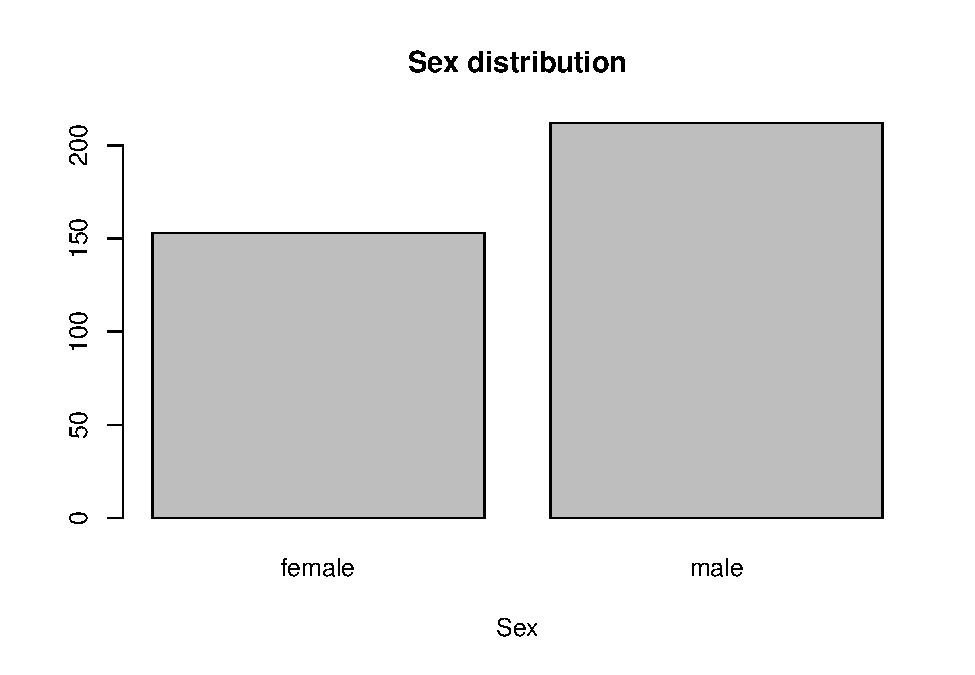
\includegraphics{_main_files/figure-latex/unnamed-chunk-62-1.pdf}

\subsection{One variable: A numerical
variable}\label{one-variable-a-numerical-variable}

Histogram

\begin{Shaded}
\begin{Highlighting}[]
\KeywordTok{hist}\NormalTok{(dataSPSS$age, }\DataTypeTok{main =} \StringTok{'Age'}\NormalTok{,}
     \DataTypeTok{xlab=}\StringTok{'Age in years'}\NormalTok{,}
     \DataTypeTok{ylab=}\StringTok{'Count'}\NormalTok{)}
\end{Highlighting}
\end{Shaded}

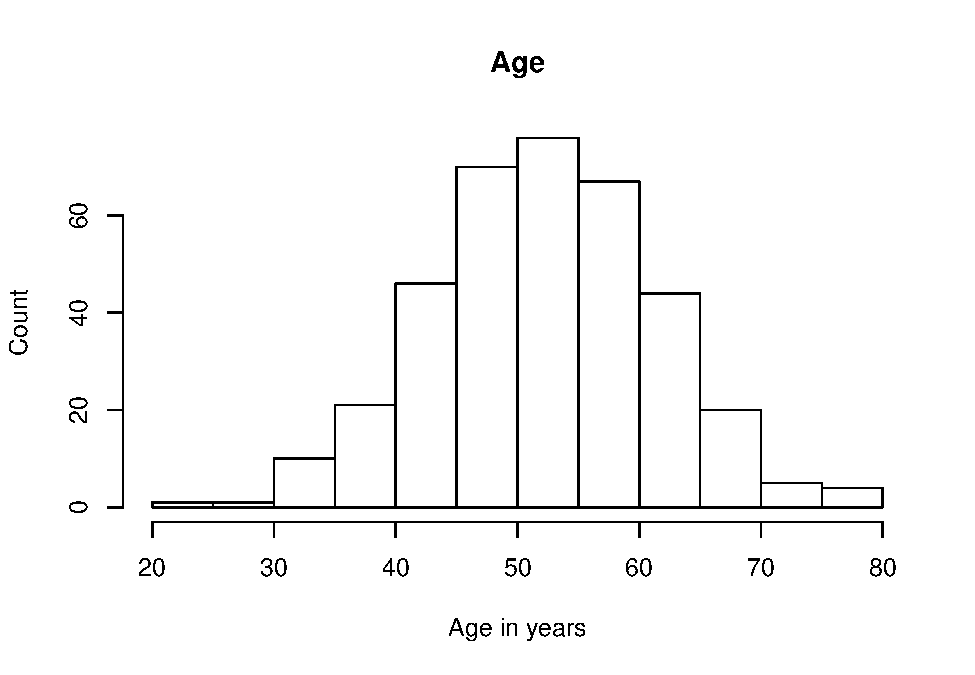
\includegraphics{_main_files/figure-latex/unnamed-chunk-63-1.pdf}

\section{Two variables}\label{two-variables}

\subsection{Two variables : A numerical with another numerical
variable}\label{two-variables-a-numerical-with-another-numerical-variable}

We will use \texttt{scatterplot} to plot

\begin{Shaded}
\begin{Highlighting}[]
\KeywordTok{plot}\NormalTok{(dataSPSS$tahundx, dataSPSS$age,}
     \DataTypeTok{main =} \StringTok{'Duration having DM VS age'}\NormalTok{,}
     \DataTypeTok{xlab =} \StringTok{'Duration of DM'}\NormalTok{, }\DataTypeTok{ylab =} \StringTok{'Age'}\NormalTok{,}
     \DataTypeTok{pch =} \DecValTok{19}\NormalTok{)}
\end{Highlighting}
\end{Shaded}

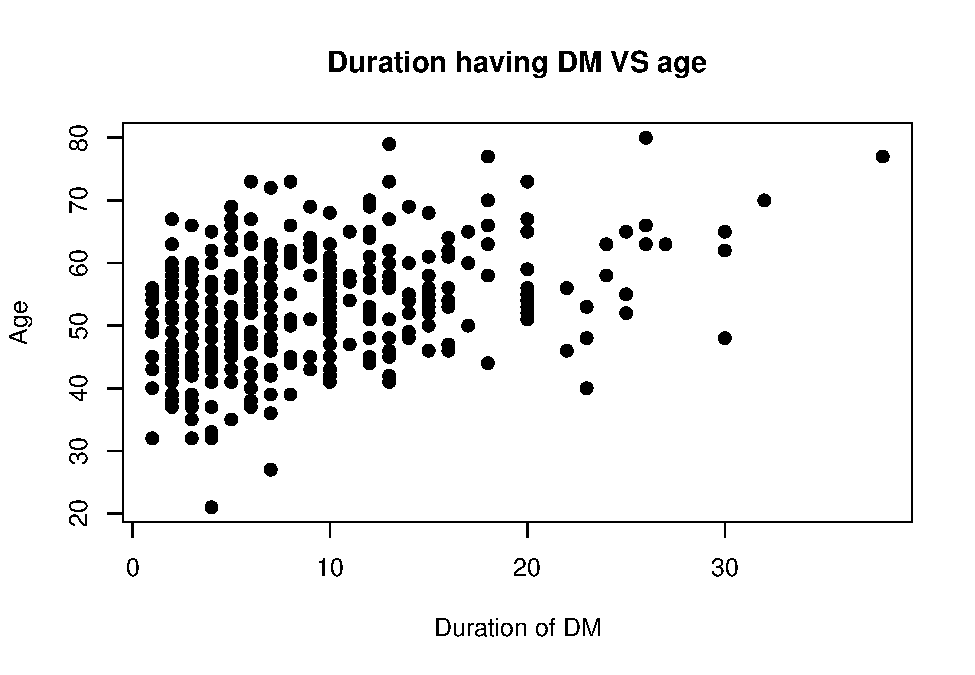
\includegraphics{_main_files/figure-latex/unnamed-chunk-64-1.pdf}

Let us make a fit line

\begin{Shaded}
\begin{Highlighting}[]
\KeywordTok{plot}\NormalTok{(dataSPSS$tahundx, dataSPSS$age,}
     \DataTypeTok{main =} \StringTok{'Duration having DM VS age'}\NormalTok{,}
     \DataTypeTok{xlab =} \StringTok{'Duration of DM'}\NormalTok{, }\DataTypeTok{ylab =} \StringTok{'Age'}\NormalTok{,}
     \DataTypeTok{pch =} \DecValTok{19}\NormalTok{)}
\KeywordTok{abline}\NormalTok{(}\KeywordTok{lm}\NormalTok{(dataSPSS$age~dataSPSS$tahundx), }\DataTypeTok{col =} \StringTok{'red'}\NormalTok{)}
\end{Highlighting}
\end{Shaded}

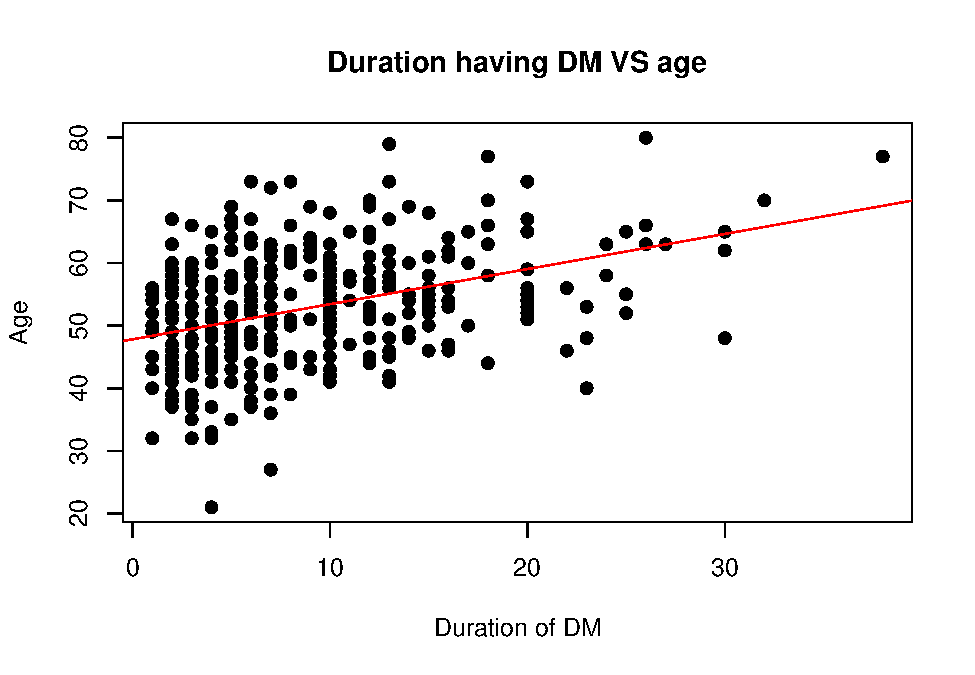
\includegraphics{_main_files/figure-latex/unnamed-chunk-65-1.pdf}

and a lowess

\begin{Shaded}
\begin{Highlighting}[]
\KeywordTok{plot}\NormalTok{(dataSPSS$tahundx, dataSPSS$age,}
     \DataTypeTok{main =} \StringTok{'Duration having DM VS age'}\NormalTok{,}
     \DataTypeTok{xlab =} \StringTok{'Duration of DM'}\NormalTok{, }\DataTypeTok{ylab =} \StringTok{'Age'}\NormalTok{,}
     \DataTypeTok{pch =} \DecValTok{19}\NormalTok{)}
\KeywordTok{lines}\NormalTok{(}\KeywordTok{lowess}\NormalTok{(dataSPSS$tahundx,dataSPSS$age), }\DataTypeTok{col =} \StringTok{'blue'}\NormalTok{)}
\end{Highlighting}
\end{Shaded}

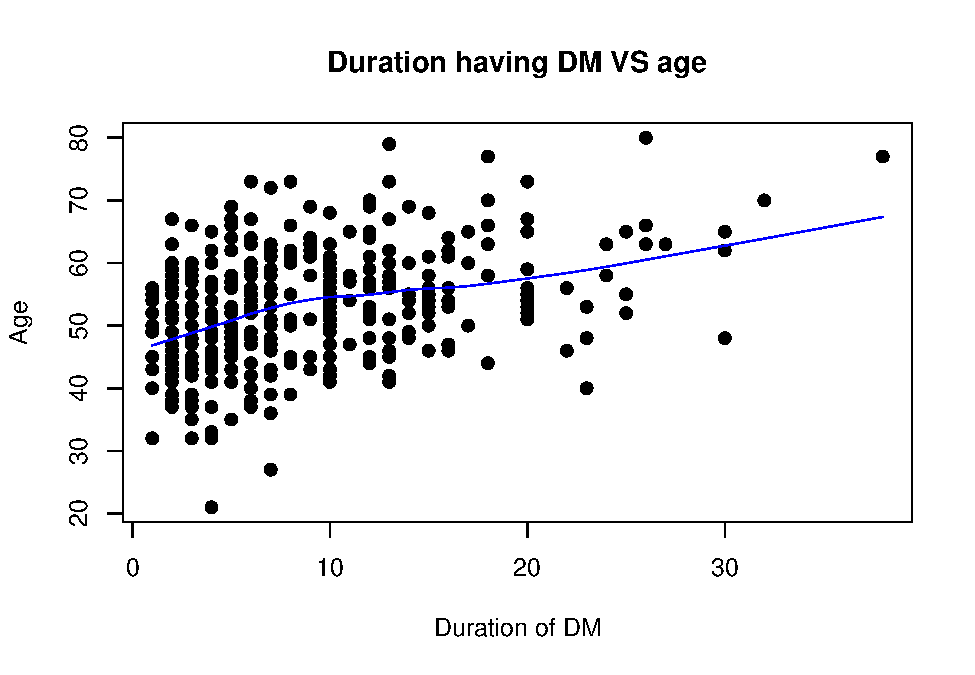
\includegraphics{_main_files/figure-latex/unnamed-chunk-66-1.pdf}

\subsection{Two variables : A categorical variable with a categorical
variable}\label{two-variables-a-categorical-variable-with-a-categorical-variable}

Now, we will plot 2 categorical variables simultanenously. First, we
will use stacked barchart

\begin{Shaded}
\begin{Highlighting}[]
\NormalTok{compl.sex<-}\KeywordTok{table}\NormalTok{(dataSPSS$complica,dataSPSS$sex)}
\NormalTok{compl.sex}
\end{Highlighting}
\end{Shaded}

\begin{verbatim}
##      
##       female male
##   no     105  120
##   yes     48   92
\end{verbatim}

\begin{Shaded}
\begin{Highlighting}[]
\KeywordTok{barplot}\NormalTok{(compl.sex,}
        \DataTypeTok{main=}\StringTok{'Complications by sex'}\NormalTok{,}
        \DataTypeTok{xlab=}\StringTok{'Sex'}\NormalTok{,}
        \DataTypeTok{col=}\KeywordTok{c}\NormalTok{(}\StringTok{'blue'}\NormalTok{,}\StringTok{'red'}\NormalTok{),}
        \DataTypeTok{legend=}\KeywordTok{c}\NormalTok{(}\StringTok{'No'}\NormalTok{,}\StringTok{'Yes'}\NormalTok{))}
\end{Highlighting}
\end{Shaded}

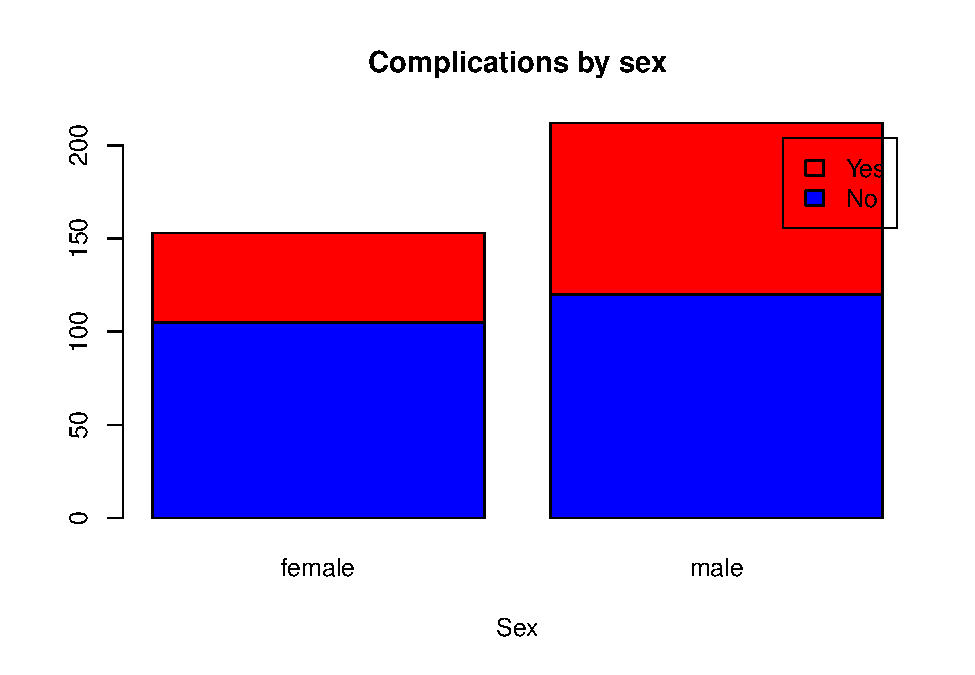
\includegraphics{_main_files/figure-latex/unnamed-chunk-67-1.pdf}

Next, we will use grouped barchart

\begin{Shaded}
\begin{Highlighting}[]
\NormalTok{compl.sex}
\end{Highlighting}
\end{Shaded}

\begin{verbatim}
##      
##       female male
##   no     105  120
##   yes     48   92
\end{verbatim}

\begin{Shaded}
\begin{Highlighting}[]
\KeywordTok{barplot}\NormalTok{(compl.sex,}
        \DataTypeTok{main =} \StringTok{'Complications according to sex'}\NormalTok{,}
        \DataTypeTok{xlab =} \StringTok{'Sex'}\NormalTok{,}
        \DataTypeTok{col =} \KeywordTok{c}\NormalTok{(}\StringTok{'blue'}\NormalTok{,}\StringTok{'red'}\NormalTok{),}
        \DataTypeTok{legend =} \KeywordTok{c}\NormalTok{(}\StringTok{'no'}\NormalTok{,}\StringTok{'yes'}\NormalTok{),}
        \DataTypeTok{beside =} \OtherTok{TRUE}\NormalTok{)}
\end{Highlighting}
\end{Shaded}

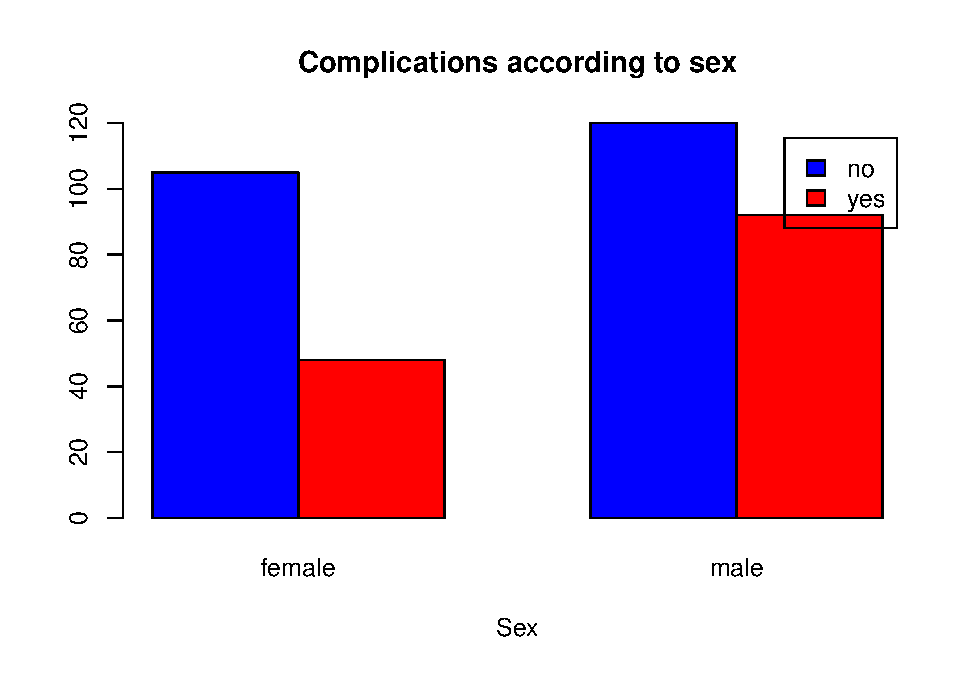
\includegraphics{_main_files/figure-latex/unnamed-chunk-68-1.pdf}

\section{Summary}\label{summary-1}

{[}summary here{]}

\chapter{Reporting results}\label{reporting-results}

Summary of chapter.

\chapter{Summary}\label{summary-2}

Summary of chapter here.

\section{What we have learned so far}\label{what-we-have-learned-so-far}

\section{Some important packages}\label{some-important-packages}

\texttt{car} \texttt{dplyr}

Example of in text citation is Xie
(\protect\hyperlink{ref-xie2015}{2015})

\chapter{References}\label{references}

\hypertarget{refs}{}
\hypertarget{ref-xie2015}{}
Xie, Yihui. 2015. \emph{Dynamic Documents with R and Knitr}. 2nd ed.
Boca Raton, Florida: Chapman; Hall/CRC. \url{http://yihui.name/knitr/}.


\end{document}
